
\documentclass[3p]{elsarticle}
\journal{}

\usepackage{graphicx}
\usepackage{amsmath}
\usepackage{amssymb}
\usepackage{amsthm}
\usepackage{latexsym}
\usepackage{bm}
\usepackage{array,supertabular}
\usepackage{color}
\usepackage{framed}
\usepackage{setspace}
\usepackage{fancyhdr}
\usepackage{stmaryrd}
\usepackage{mathrsfs}
\usepackage{mdframed}
\usepackage{url}
\usepackage{ctex}
\usepackage{algorithm}
\usepackage{algpseudocode}
\usepackage{subfigure}

\SetSymbolFont{stmry}{bold}{U}{stmry}{m}{n}

\newtheorem{defi}{Definition}
\newtheorem{lemma}{Lemma}
\newtheorem{proposition}{Proposition}
\newtheorem{remark}{Remark}

\numberwithin{equation}{section}

\newenvironment{myenv}[1]
{\mdfsetup{
		frametitle={\colorbox{white}{\space#1\space}},
		innertopmargin=10pt,
		frametitleaboveskip=-\ht\strutbox,
		frametitlealignment=\center
	}
	\begin{mdframed}
	}
	{\end{mdframed}}

\begin{document}
	
	\begin{frontmatter}
		
		\title{\textbf{MAE 5032 HPC Final Project --  the transient heat equation in a one-dimensional (1D) domain}}
		\author{Jiayi Huang}
		
		\begin{abstract}
			本文利用有限差分法计算热方程的数值解,在一个一维热方程的具体问题中,使用显示欧拉法和隐式欧拉法分别求解,两种求解均基于PETsC库。根据逐步加细的网格和逐步减小的时间步长,分析并计算了截断误差如何依赖于网格间距和时间步长,并给出理论预测。
		\end{abstract}
		
		\begin{keyword}
			 Finite difference method, Explicit Euler and Implicit Euler methods
		\end{keyword}
	\end{frontmatter}
	
	\section{Introduction}
    首先列出要求解的一维传热问题
    
    \begin{aligned}
	\rho c \frac{\partial u}{\partial t}-\kappa \frac{\partial^{2} u}{\partial x^{2}} &=f & & \text { on } \Omega \times(0, T) \\
	u &=g & & \text { on } \Gamma_{g} \times(0, T) \\
	\kappa \frac{\partial u}{\partial x} n_{x} &=h & & \text { on } \Gamma_{h} \times(0, T) \\
	\left.u\right|_{t=0} &=u_{0} & & \text { in } \Omega . 
\end{aligned}

    其中 $u = u(x,t)$ 是要求解的 $t$ 时刻,$x$ 位置处的温度。可以画出下面的示意网格。
    
    \begin{figure}[h]
	\begin{center}
		\begin{tabular}{c}
			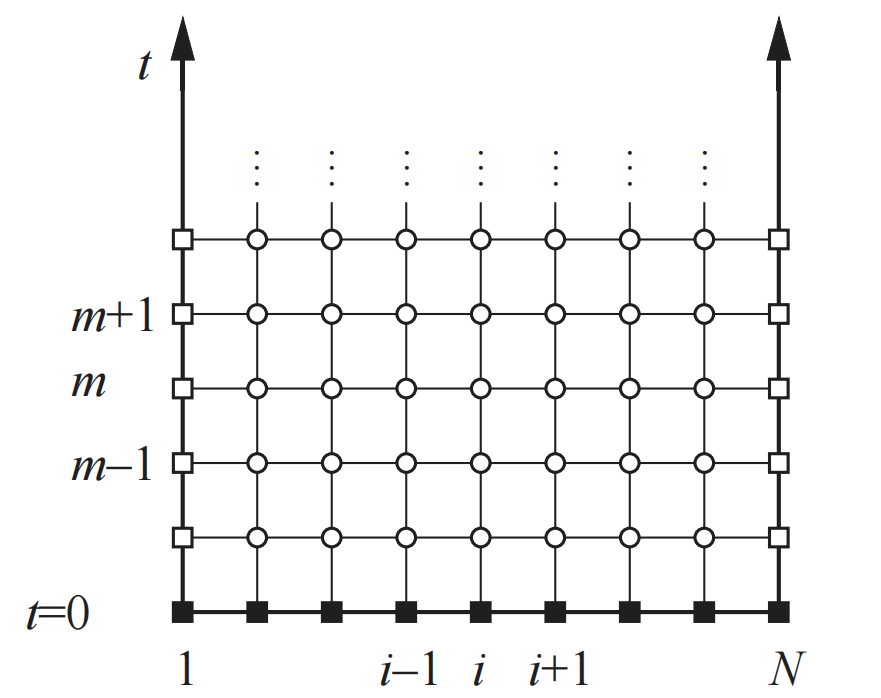
\includegraphics[angle=0, scale=0.25]{./figures/mesh.png}
		\end{tabular}
	\end{center}
	\caption{解一维热方程的示意网格,实心方块代表已知位置,空心的则代表用有限差分近似的位置}
	\label{fig:illustration-mesh}
    \end{figure}
    
    
    \begin{figure}[h]
    	\begin{center}
    		\begin{tabular}{c}
    			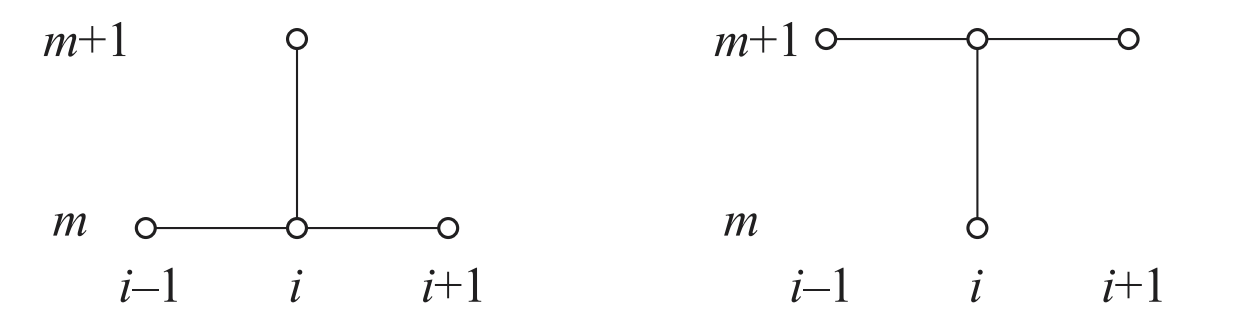
\includegraphics[angle=0, scale=0.25]{./figures/compute_molecules.png}
    		\end{tabular}
    	\end{center}
    	\caption{关于有限差分的计算子,左边是Explicit Euler,右边是Implicit Euler}
    	\label{fig:illustration-molecules}
    \end{figure}

    根据上面的差分算子示意图,可以推导出下面的两个 Explicit Euler 和 Implicit Euler 迭代公式。
        
	\begin{equation}
		u_{i}^{m+1}=\alpha u_{i+1}^{m}+(1-2 \alpha) u_{i}^{m}+\alpha u_{i-1}^{m} + \beta \cdot f
	\end{equation}

	\begin{equation}
	    u_{i}^{m-1} = -\alpha u_{i+1}^{m}+(1+2 \alpha) u_{i}^{m}-\alpha u_{i-1}^{m} - \beta \cdot f
	\end{equation}

    其中 $ \alpha =  \kappa \beta / \Delta x^{2} $ , $ \beta = \Delta t / \rho c  $ , \\ 代入边界条件 $f = \sin (l \pi x), \quad u_{0} = e^{x}, \quad u(0, t) = u(1, t) = 0, \quad \kappa = 1.0$ ,进而获得对应的三对角迭代矩阵,再套用之前作业中完成的解三对角矩阵程序进行求解。
    
    \section{Code development}
    
    \subsection{Codes for explicit Euler and implicit Euler methods}
    
    这里附上设置 $ \alpha $ , $ \beta  $ 等等常数参数,以及设置系数矩阵Matrix A的代码
    
    \begin{figure}[h]
    	\begin{center}
    		\begin{tabular}{c}
    			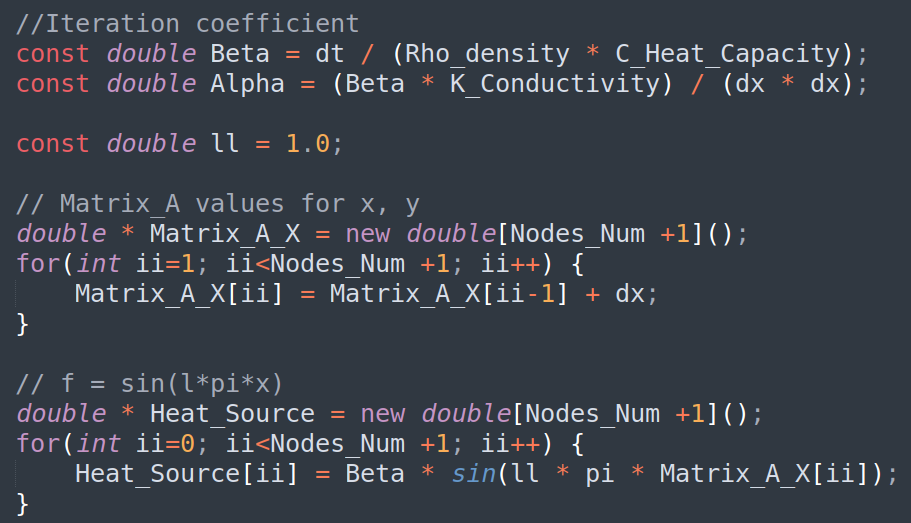
\includegraphics[angle=0, scale=0.25]{./figures/matrix_coefficient.png}
    		\end{tabular}
    	\end{center}
    	\caption{$ \alpha $ , $ \beta  $ 以及热源初始条件的设置}
    	\label{fig:illustration-matrix_coefficient}
    \end{figure}

    \begin{figure}[h]
    	\begin{center}
    		\begin{tabular}{c}
    			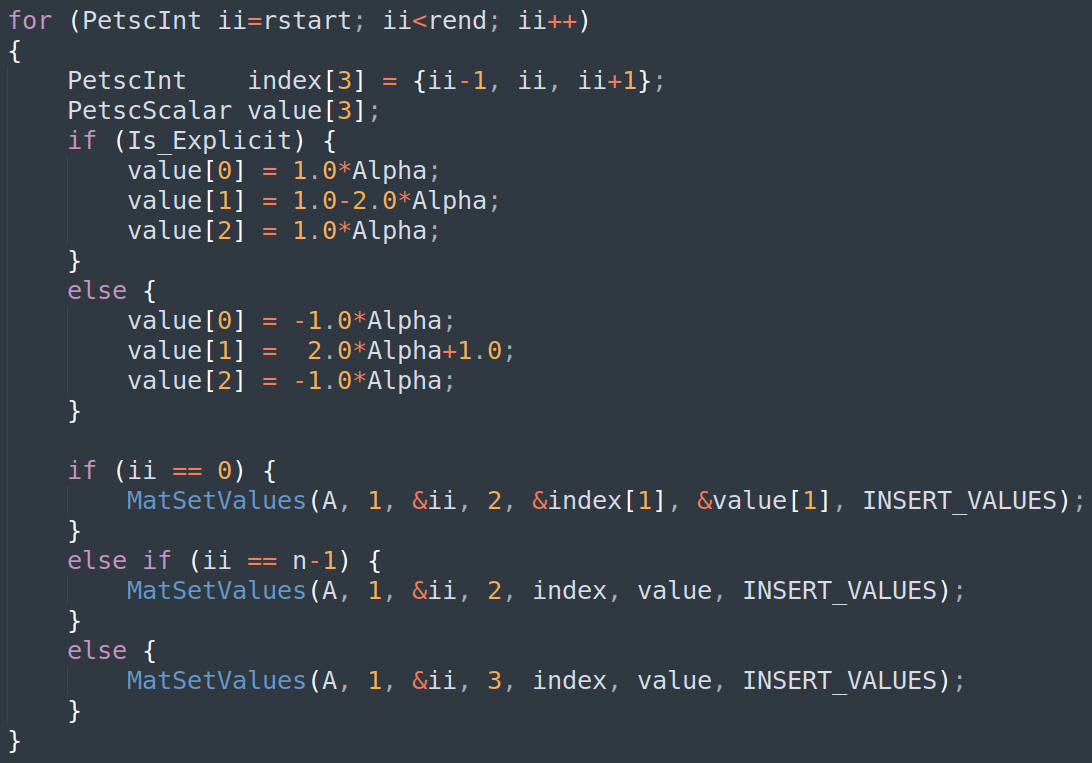
\includegraphics[angle=0, scale=0.18]{./figures/matrix_each_value.png}
    		\end{tabular}
    	\end{center}
    	\caption{$ Matrix\_A $ 中的各个元素的值的设置}
    	\label{fig:illustration-matrix_each_value}
    \end{figure}

    如上图代码中所示,使用了 $ Bool $ 变量 $ Is\_Explicit $ 来区分显式欧拉和隐式欧拉
    
    \begin{figure}[h]
    	\begin{center}
    		\begin{tabular}{c}
    			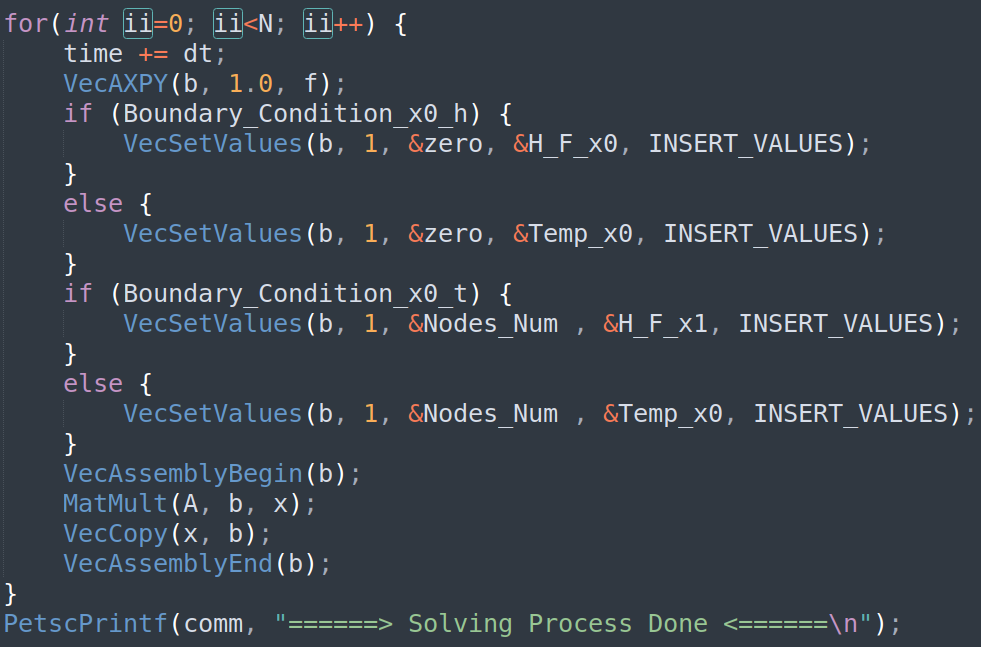
\includegraphics[angle=0, scale=0.205]{./figures/Explicit_Euler.png}
    		\end{tabular}
    	\end{center}
    	\caption{$ Explicit\_Euler $ $ Codes $}
    	\label{fig:illustration-Explicit_Euler}
    \end{figure}
    
    \begin{figure}[h]
    	\begin{center}
    		\begin{tabular}{c}
    			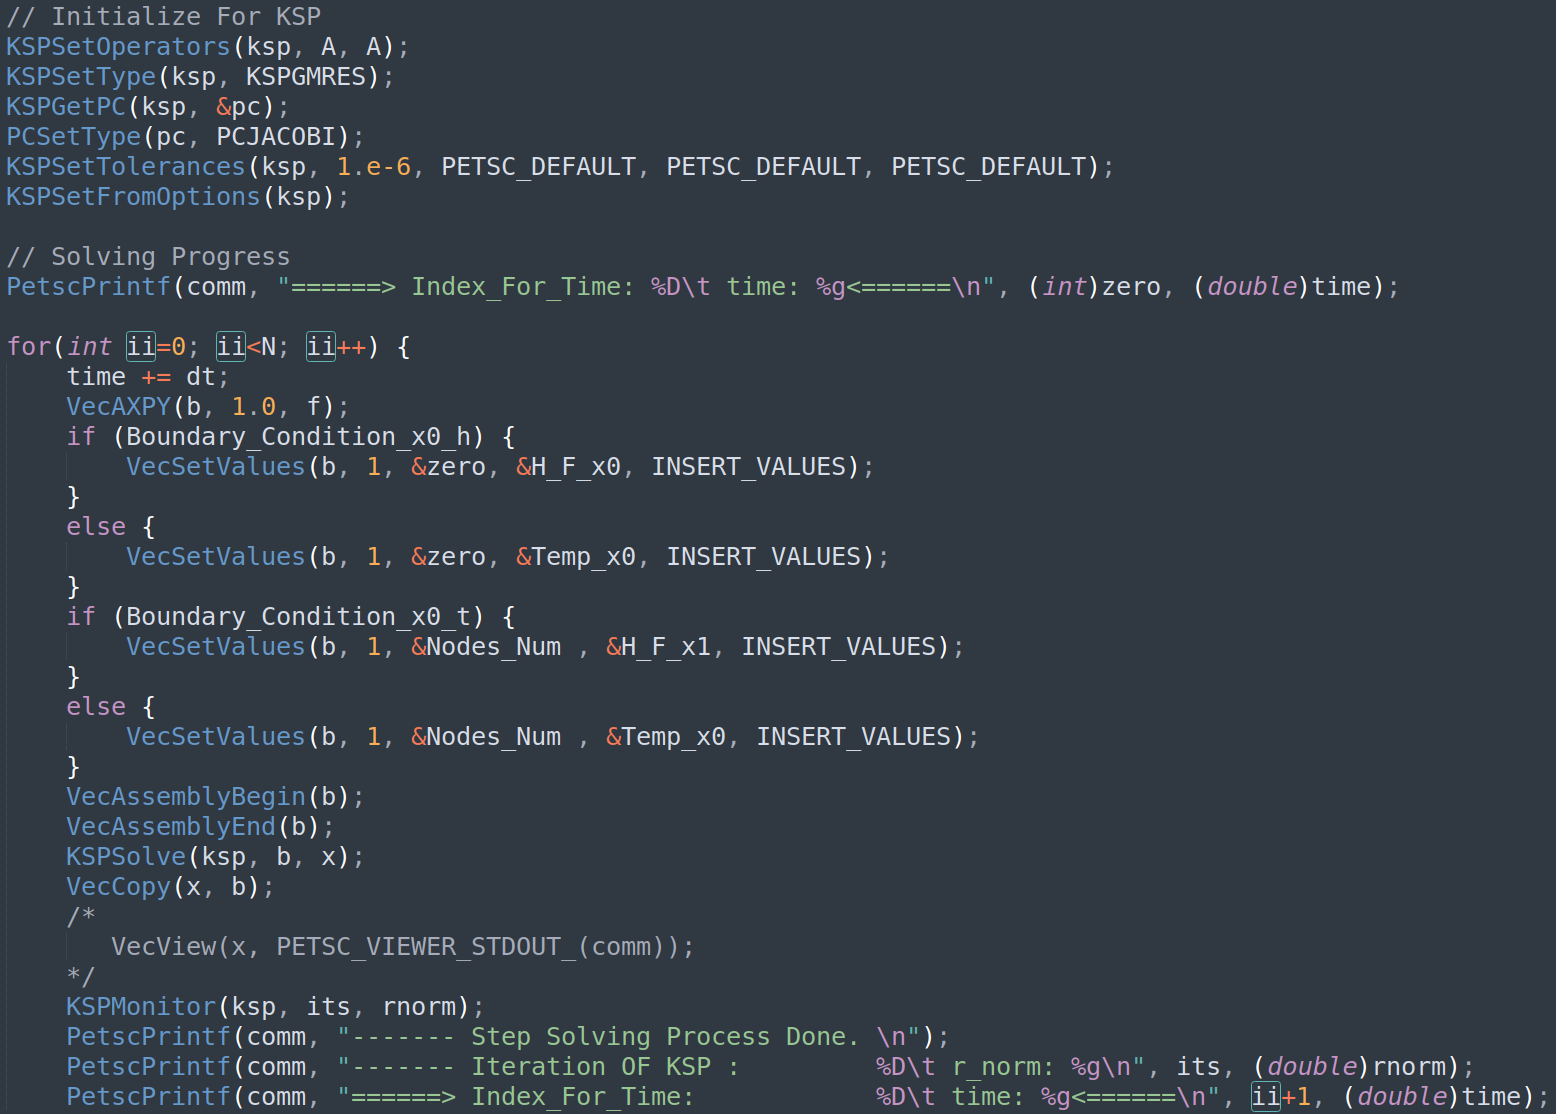
\includegraphics[angle=0, scale=0.13]{./figures/Implicit_Euler.png}
    		\end{tabular}
    	\end{center}
    	\caption{$ Implicit\_Euler $ $ Codes $}
    	\label{fig:illustration-Implicit_Euler}
    \end{figure}
    
    
    如 Figure \ref{fig:illustration-Implicit_Euler} ($ Implicit\_Euler $) 图代码中,区别于显式迭代,隐式迭代在每个时间步需要解一个线性方程组,可以设置迭代方法和预条件子。
    \clearpage
    \subsection{The stability property and comparison with exact solution}
    
    \subsubsection{Explicit stability}
    
    根据《微分方程数值解》(戴嘉尊)中的结论
    \begin{equation}
    	\lambda_{j}=1-2 \alpha+2 \alpha \cos (j \pi \Delta x)=1-4 \alpha \sin ^{2} \frac{j \pi \Delta x}{2} \quad(j=1,2, \cdots, M-1)
    \end{equation}
    矩阵的特征值要小于 1 ,也即 $ \alpha =  \frac{\kappa \Delta t}{ \rho c \Delta x^{2}} < \frac{1}{2} $,这是古典显式差分格式稳定的充分必要条件。
    在这里通过设置 Nodes\_Num = 10  , 可知 $ \Delta x^{2} = 0.01 $ , 取 $ \kappa = \rho = c = 1 $ , 推导出需要设置 $ \Delta t \le   0.005 $ 才能收敛。
    
    经过实验并做图,可以发现 $ \le   0.005 $ 的黑线和橙线是稳定的,而红线、蓝线和黄线偏离的程度依次爆炸式增大。这符合之前的稳定性理论分析。可以看到实现的显式算法代码能够把解迭代到离精确解误差很小的范围内。
    
    \begin{figure}[h]
    	\begin{center}
    		\begin{tabular}{c}
    			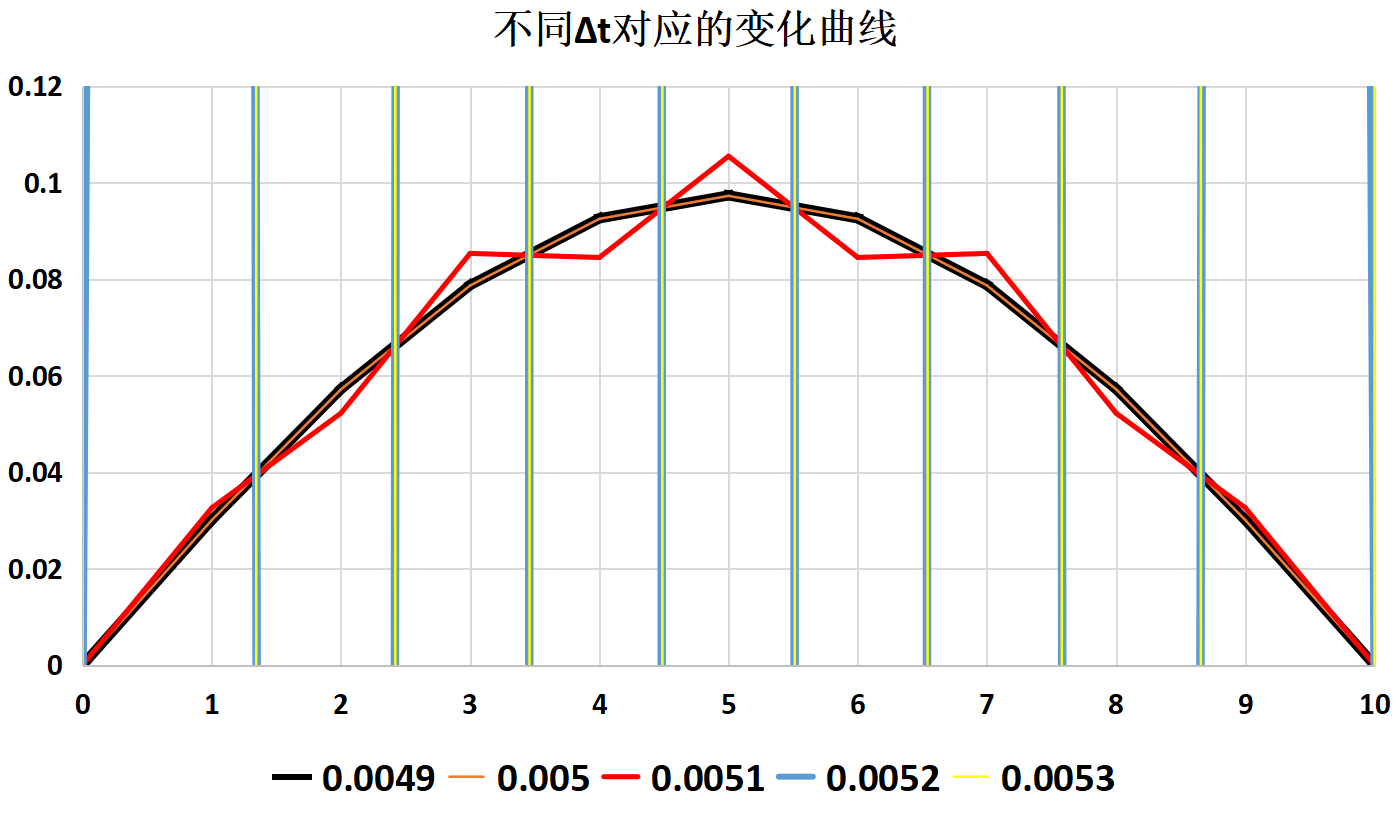
\includegraphics[angle=0, scale=0.15]{./figures/Explicit_Stablity.png}
    			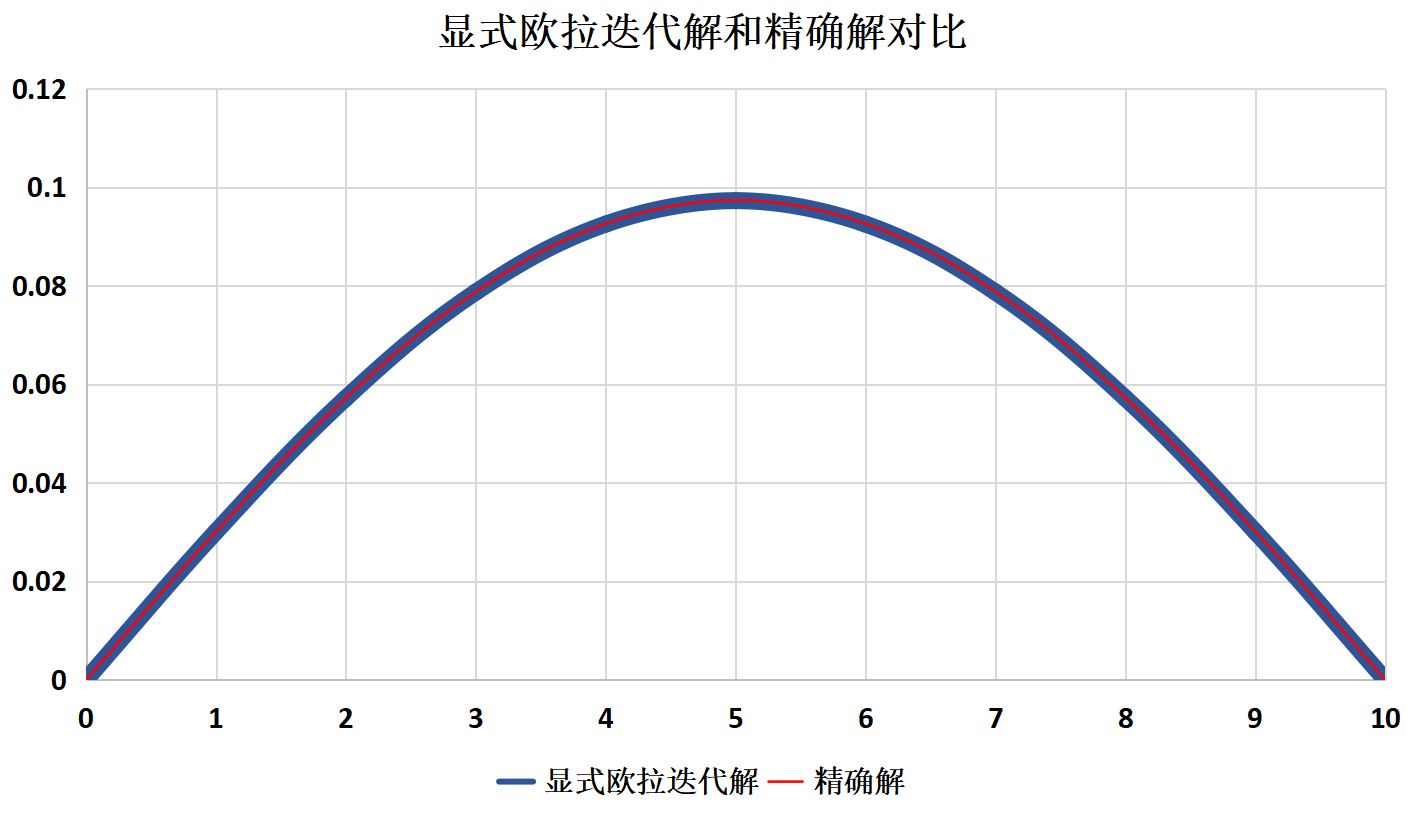
\includegraphics[angle=0, scale=0.15]{./figures/Explicit_Stablity_Compare.png}
    		\end{tabular}
    	\end{center}
    	\caption{显式欧拉迭代法的稳定性分析,$\le$ 0.005稳定}
    	\label{fig:illustration-Explicit_Stablity}
    \end{figure}
    
    \clearpage
    \subsubsection{Implicit stability}
    
    根据《微分方程数值解》(戴嘉尊)中的结论和误差分析公式,可以知道隐式结构无条件稳定,从下图中同样能够看出,隐式欧拉迭代法能稳定迭代到离精确解很小的范围内。
    \begin{equation}
    	\left|e^{\sigma \Delta t}\right|=\left|\frac{1}{1+2 \beta[1-\cos (\kappa \Delta x)]}\right| \leq 1
    \end{equation}
    \begin{figure}[h]
    	\begin{center}
    		\begin{tabular}{c}
    			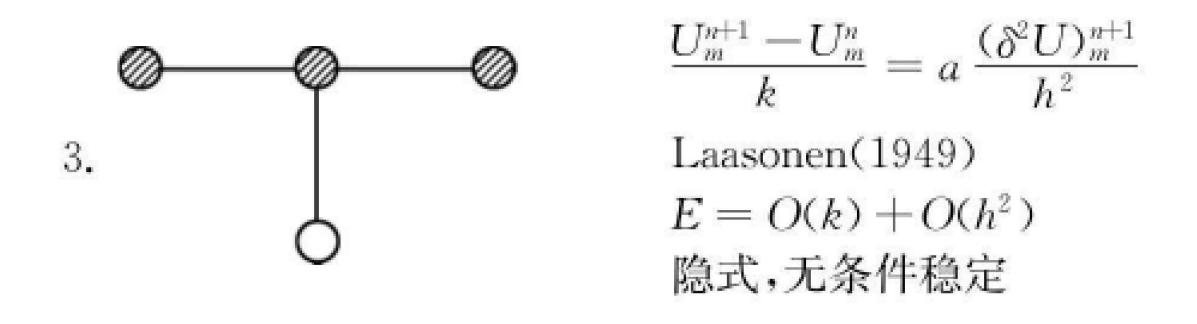
\includegraphics[angle=0, scale=0.25]{./figures/Implicit_Stablity.png}
    		\end{tabular}
    	\end{center}
    	\caption{隐式欧拉迭代法的稳定性分析,无条件稳定}
    	\label{fig:illustration-Implicit_Stablity}
    \end{figure}
    
    
    \begin{figure}[h]
    	\begin{center}
    		\begin{tabular}{c}
    			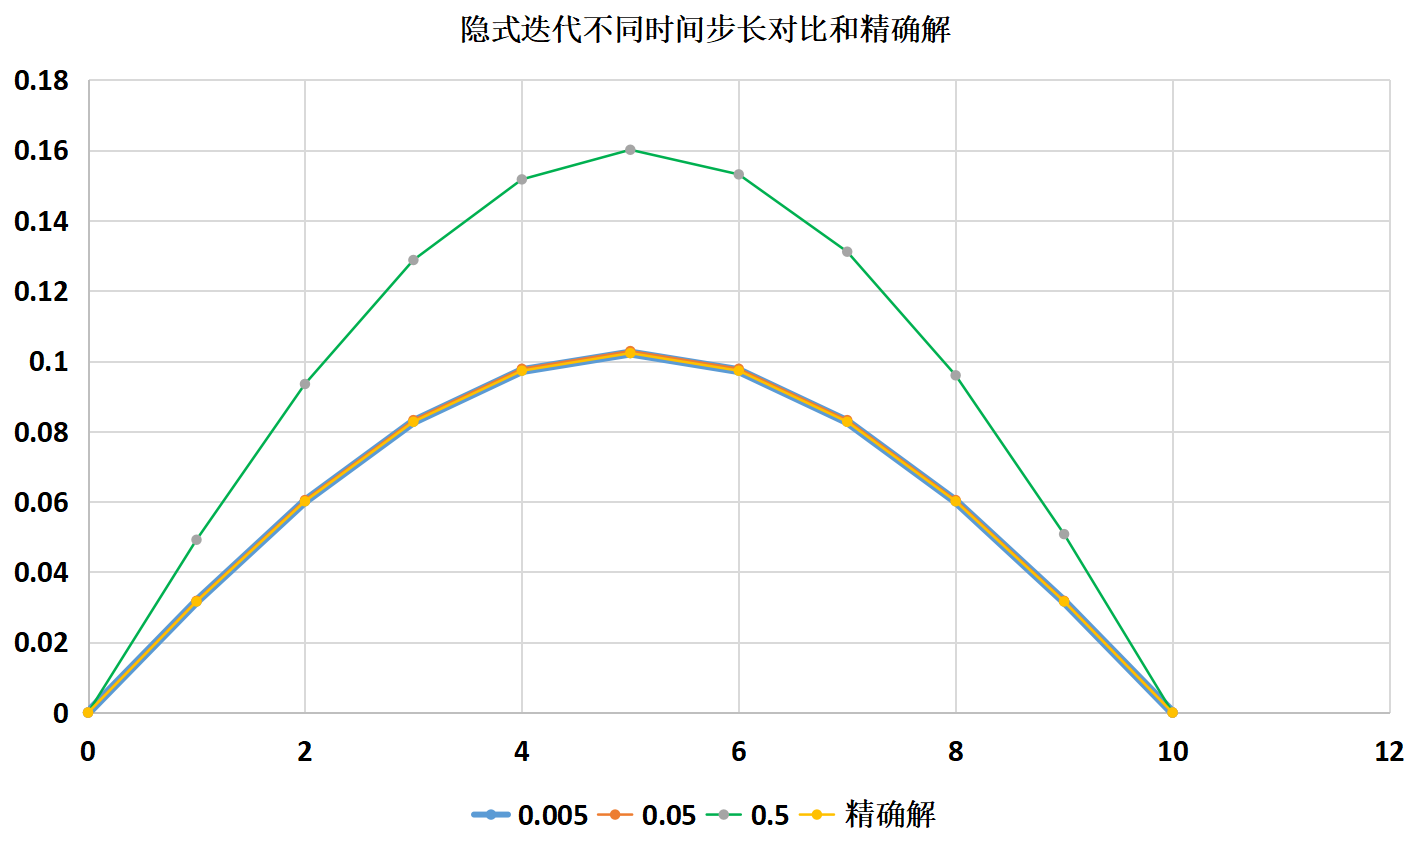
\includegraphics[angle=0, scale=0.25]{./figures/Implicit_Euler_Stability.png}
    		\end{tabular}
    	\end{center}
    	\caption{隐式欧拉迭代法的不同时间步长对比,可以看出0.05时即可达到较好精度}
    	\label{fig:illustration-Implicit_Euler_Stability}
    \end{figure}

    \clearpage

    \subsection{The restart facility using HDF5}
    
    \begin{figure}[h]
    	\begin{center}
    		\begin{tabular}{c}
    			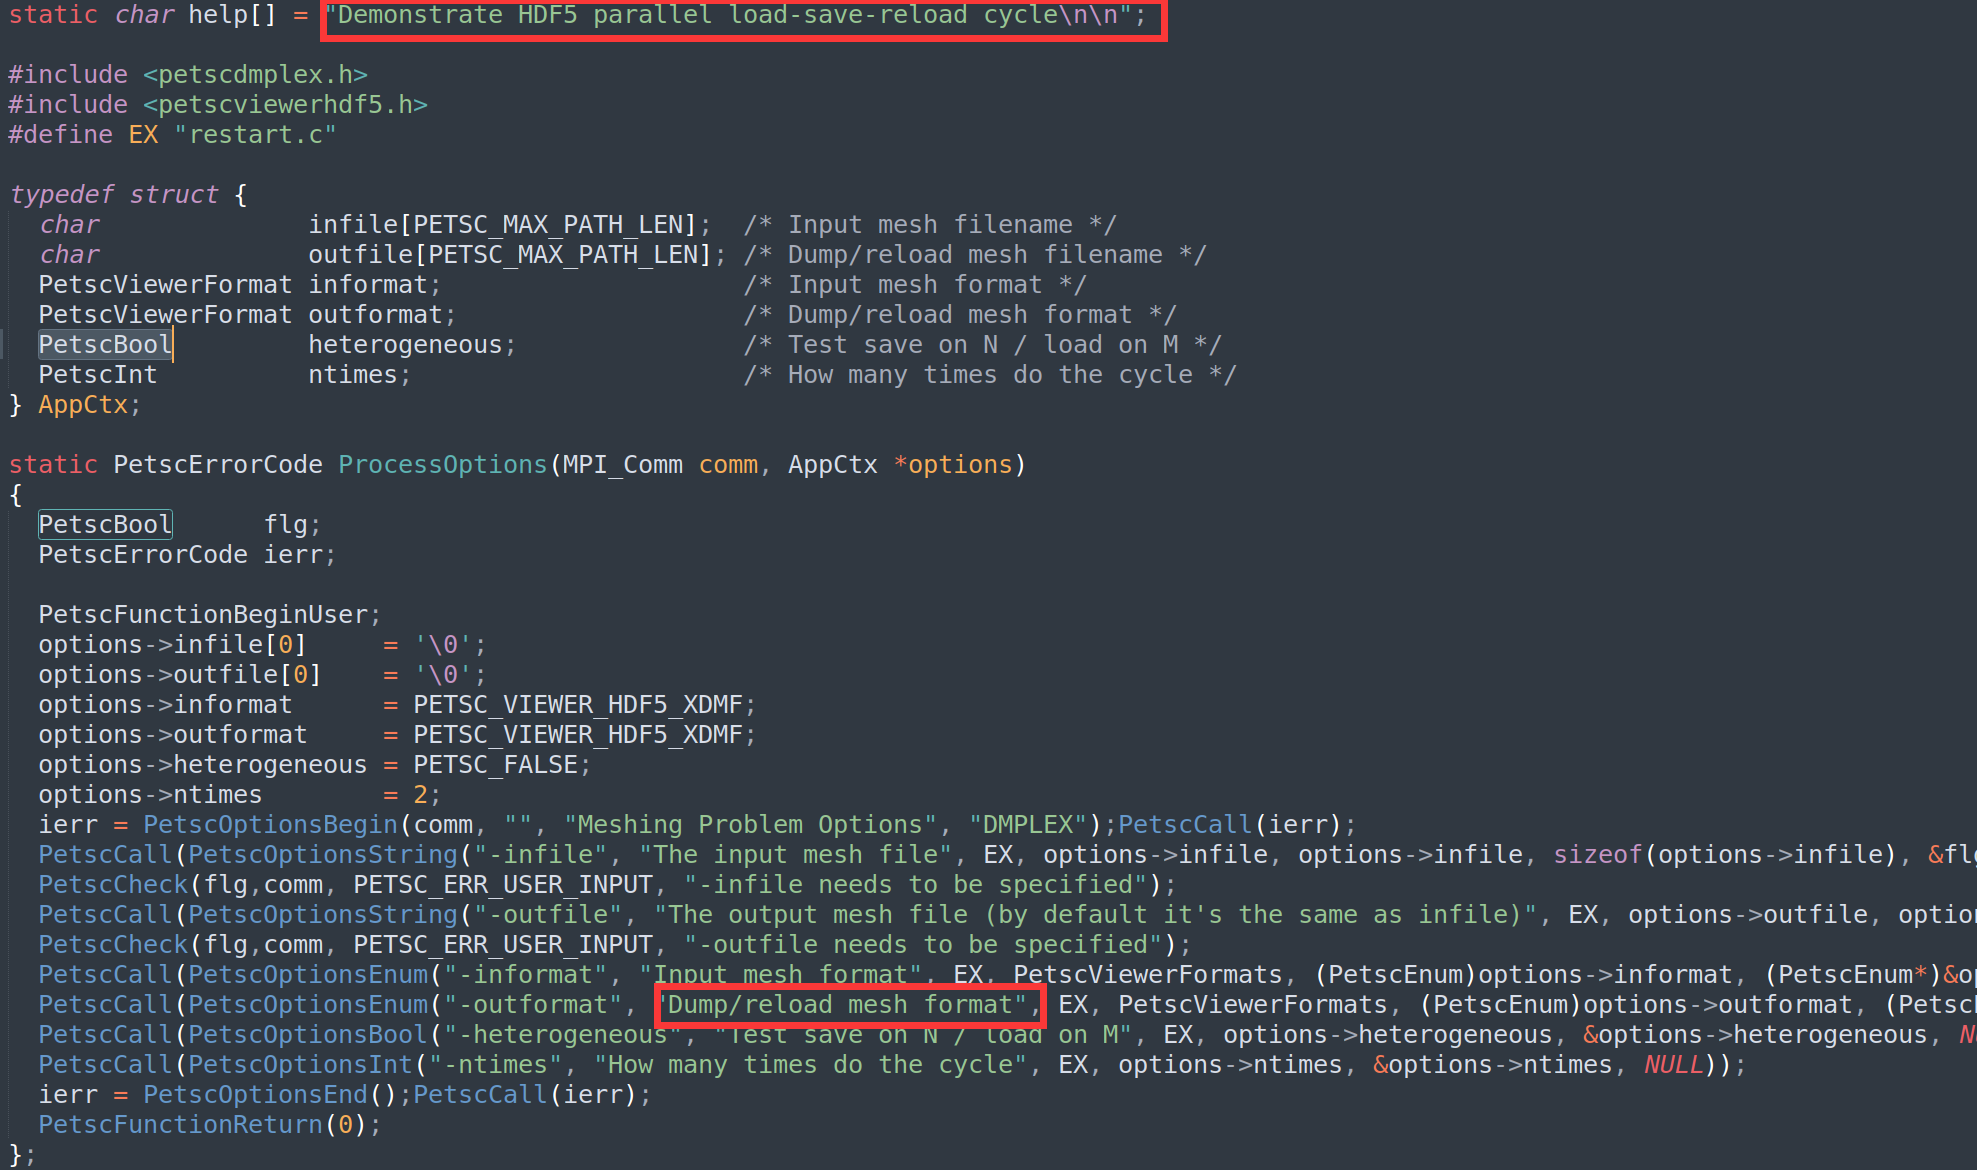
\includegraphics[angle=0, scale=0.16]{./figures/restart.png}
    		\end{tabular}
    	\end{center}
    	\caption{PETsC提供的HDF5并行重启示例程序}
    	\label{fig:illustration-restart}
    \end{figure}
    
    
    \begin{figure}[h]
    	\begin{center}
    		\begin{tabular}{c}
    			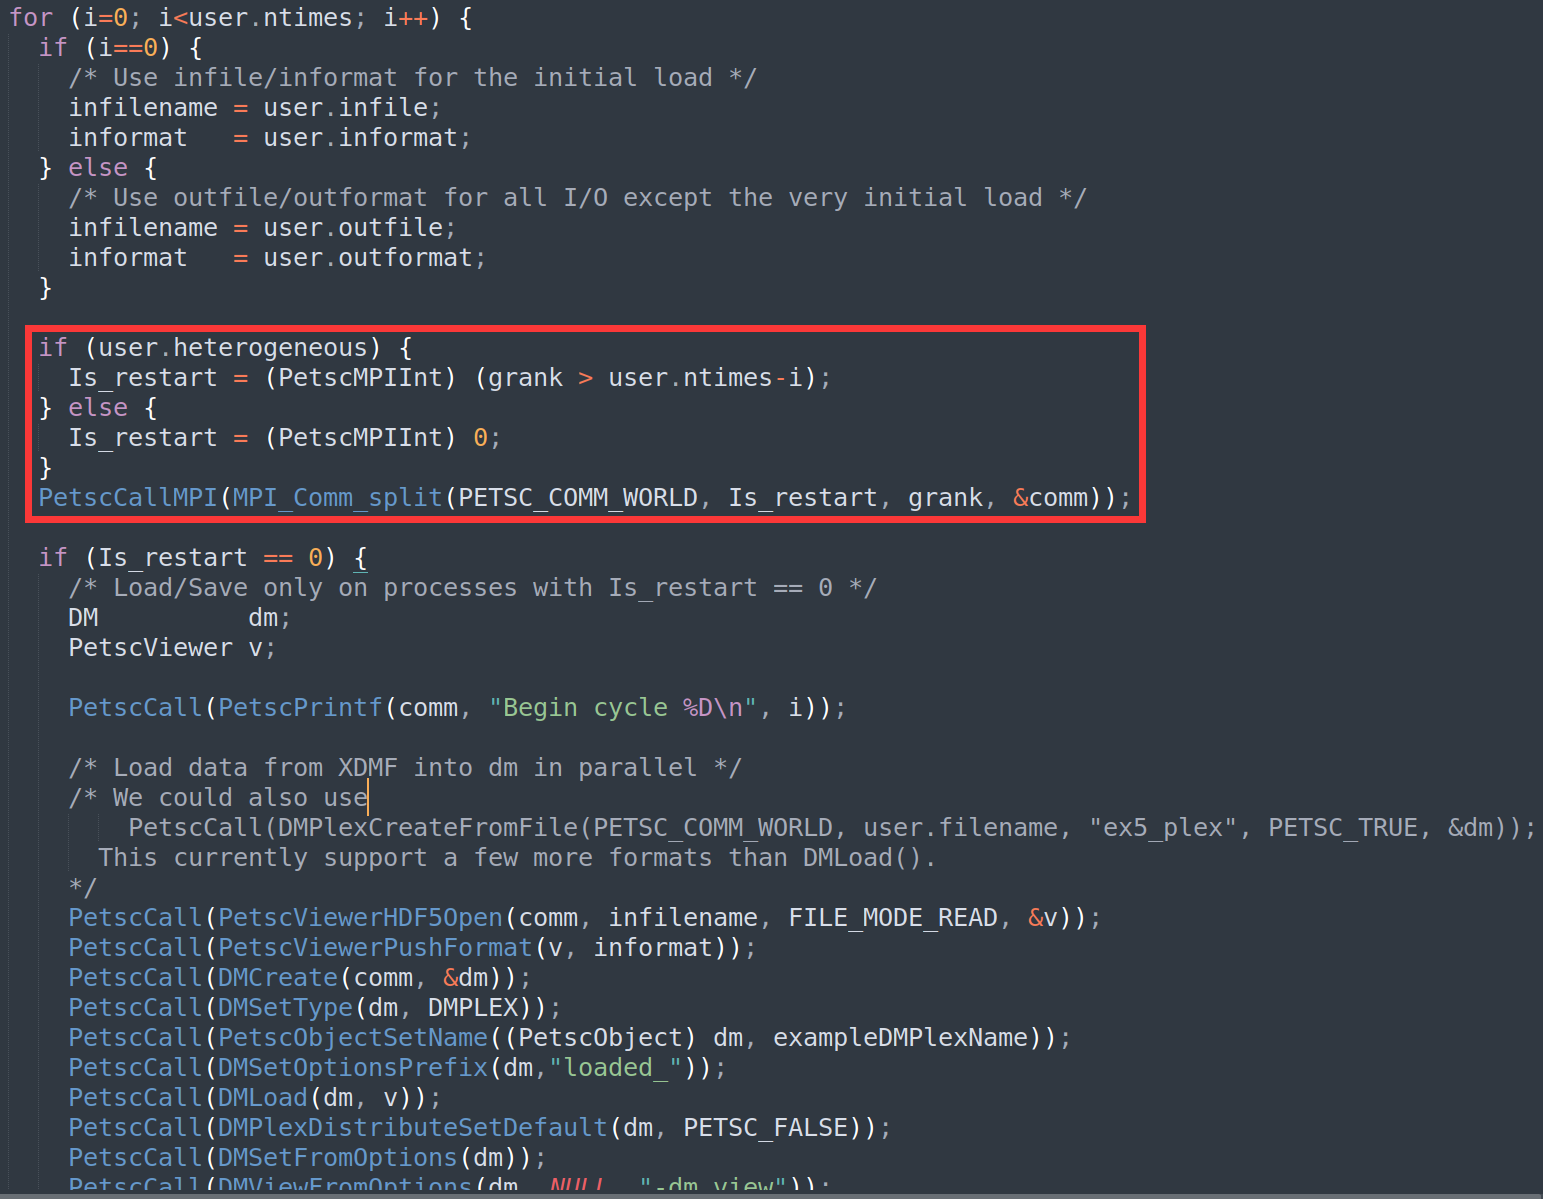
\includegraphics[angle=0, scale=0.16]{./figures/restart1.png}
    		\end{tabular}
    	\end{center}
    	\caption{具体代码细节,根据输入的PetscBool来判别是否进行断点重启运算}
    	\label{fig:illustration-restart1}
    \end{figure}
    经过测试,可以完成断点恢复,不用重新从头计算。
    \clearpage
    \subsection{Defensive manner}
    
    如下面的PETsC手册和代码图片所示,采用ierr和PetscCall来进行防御性编程;
    
    采用-Wall来找到提示警告的地方来进行防御性编程;
    
    用assert来找到变量异常的地方来进行防御性编程,前面稳定性分析要求显式欧拉需要 $ \alpha \le 0.5 $ 。 
    
    \begin{figure}[h]
    	\begin{center}
    		\begin{tabular}{c}
    			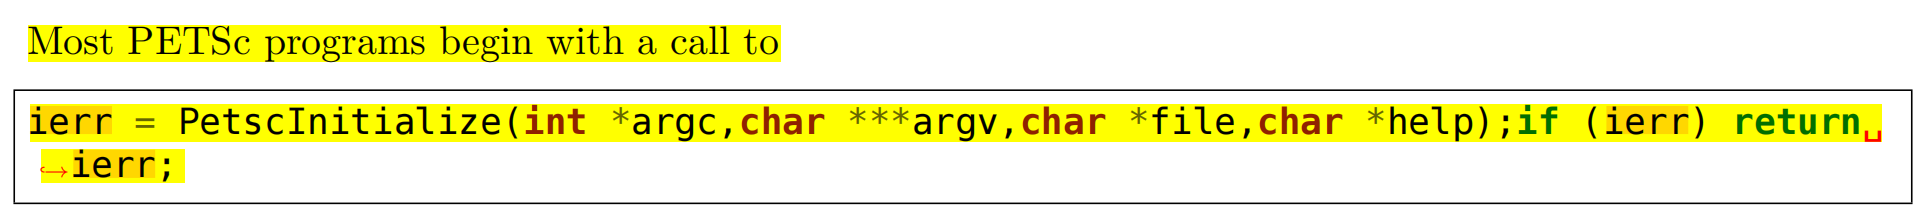
\includegraphics[angle=0, scale=0.16]{./figures/ierr.png}
    			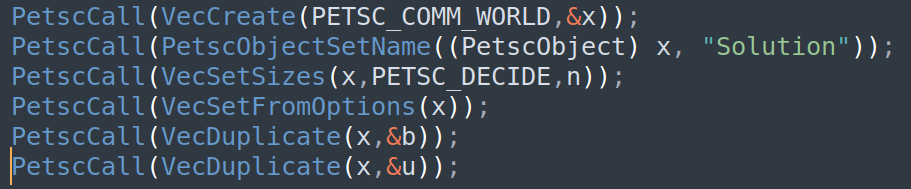
\includegraphics[angle=0, scale=0.20]{./figures/petsccall.png}
    		\end{tabular}
    	\end{center}
    	\caption{使用ierr来侦测错误 , 使用PetscCall来找到出错的地方}
    	\label{fig:illustration-ierr}
    \end{figure}
        
    \begin{figure}[h]
    	\begin{center}
    		\begin{tabular}{c}
    			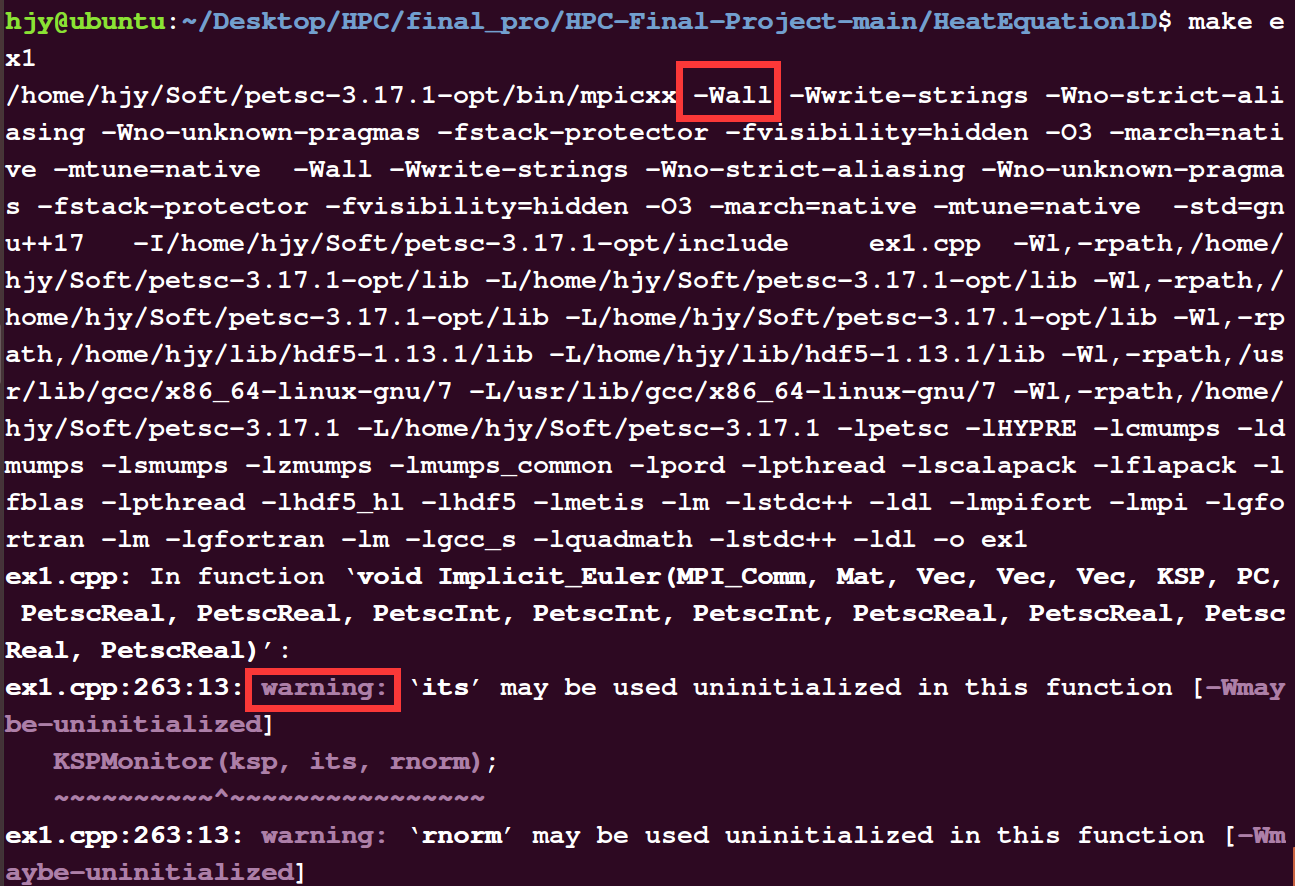
\includegraphics[angle=0, scale=0.16]{./figures/warning.png}
    			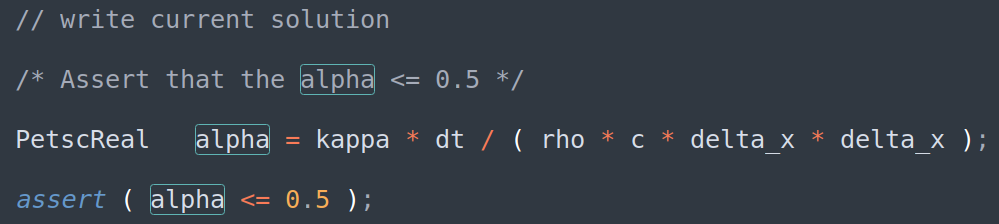
\includegraphics[angle=0, scale=0.30]{./figures/assert.png}
    		\end{tabular}
    	\end{center}
    	\caption{使用-Wall来找到提示警告的地方 , 使用assert来找到变量异常的地方}
    	\label{fig:illustration-warning}
    \end{figure}

    \clearpage
    \subsection{Compiling}
    
    \begin{figure}[h]
    	\begin{center}
    		\begin{tabular}{c}
    			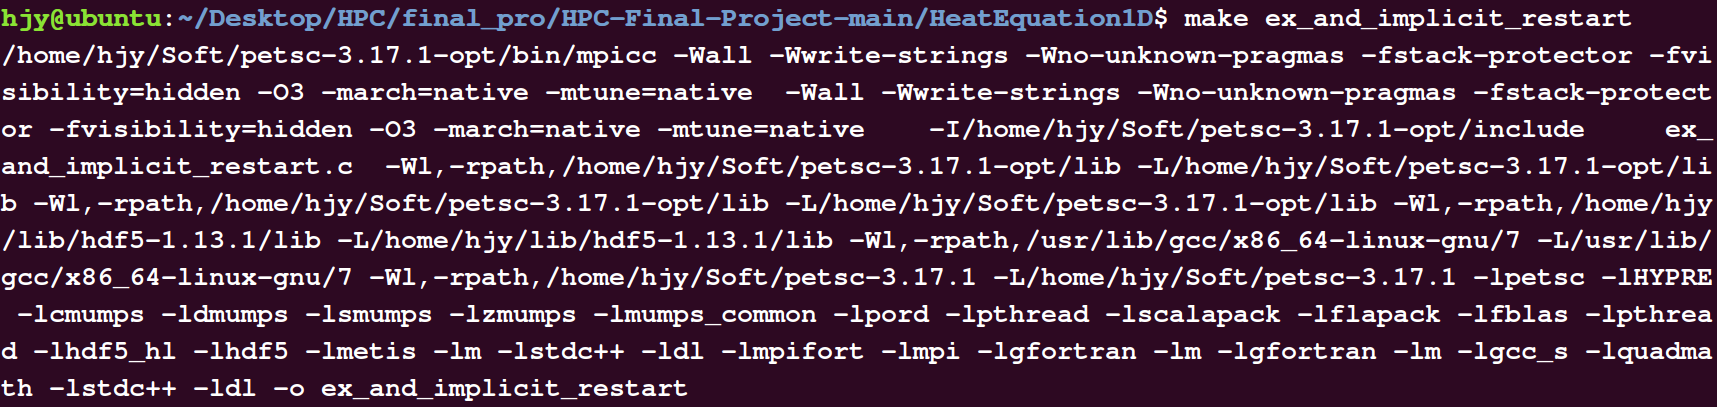
\includegraphics[angle=0, scale=0.28]{./figures/compile.png}
    		\end{tabular}
    	\end{center}
    	\caption{使用PETsC里面自带的tutorial包含的makefile,方便快捷}
    	\label{fig:illustration-compile}
    \end{figure}
    
    \subsection{Profiling analysis}
    
    \begin{figure}[h]
    	\begin{center}
    		\begin{tabular}{c}
    			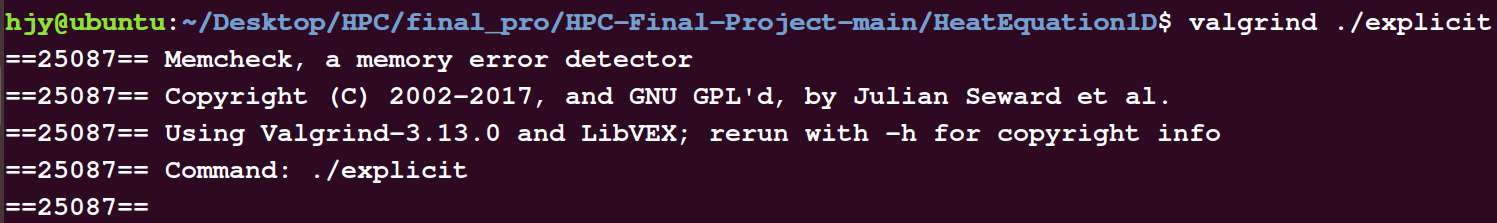
\includegraphics[angle=0, scale=0.175]{./figures/valgrind1.png}
    			
    			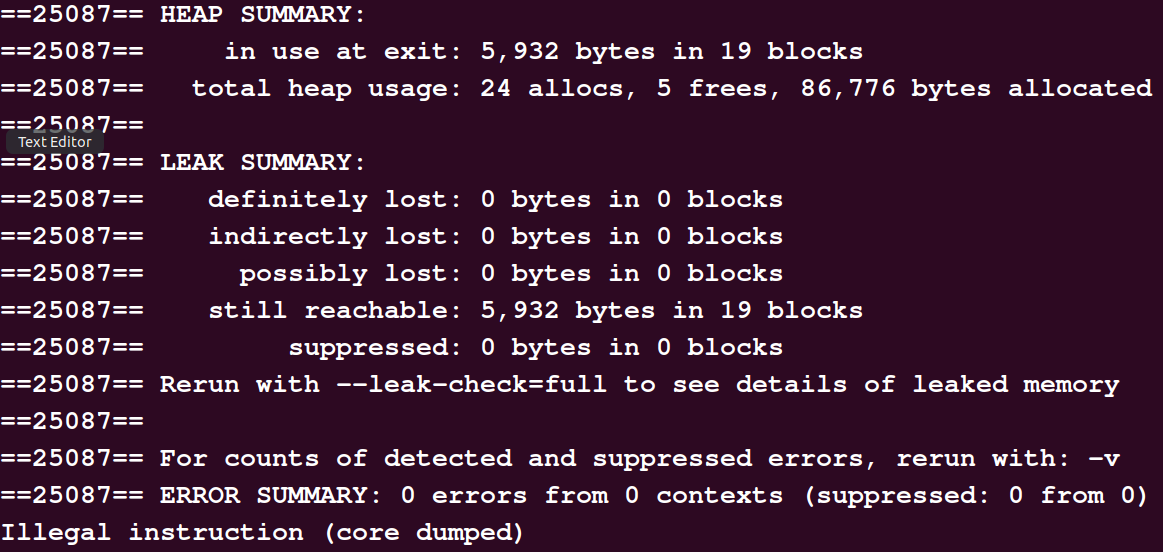
\includegraphics[angle=0, scale=0.175]{./figures/valgrind2.png}
    		\end{tabular}
    	\end{center}
    	\caption{使用valgrind进行Profiling,寻找性能瓶颈,提高运行效率}
    	\label{fig:illustration-profiling}
    \end{figure}
    从上面valgrind分析截图中可以看出没有内存泄漏,但是堆没有及时释放。

    \begin{figure}[h]
    	\begin{center}
    		\begin{tabular}{c}
    			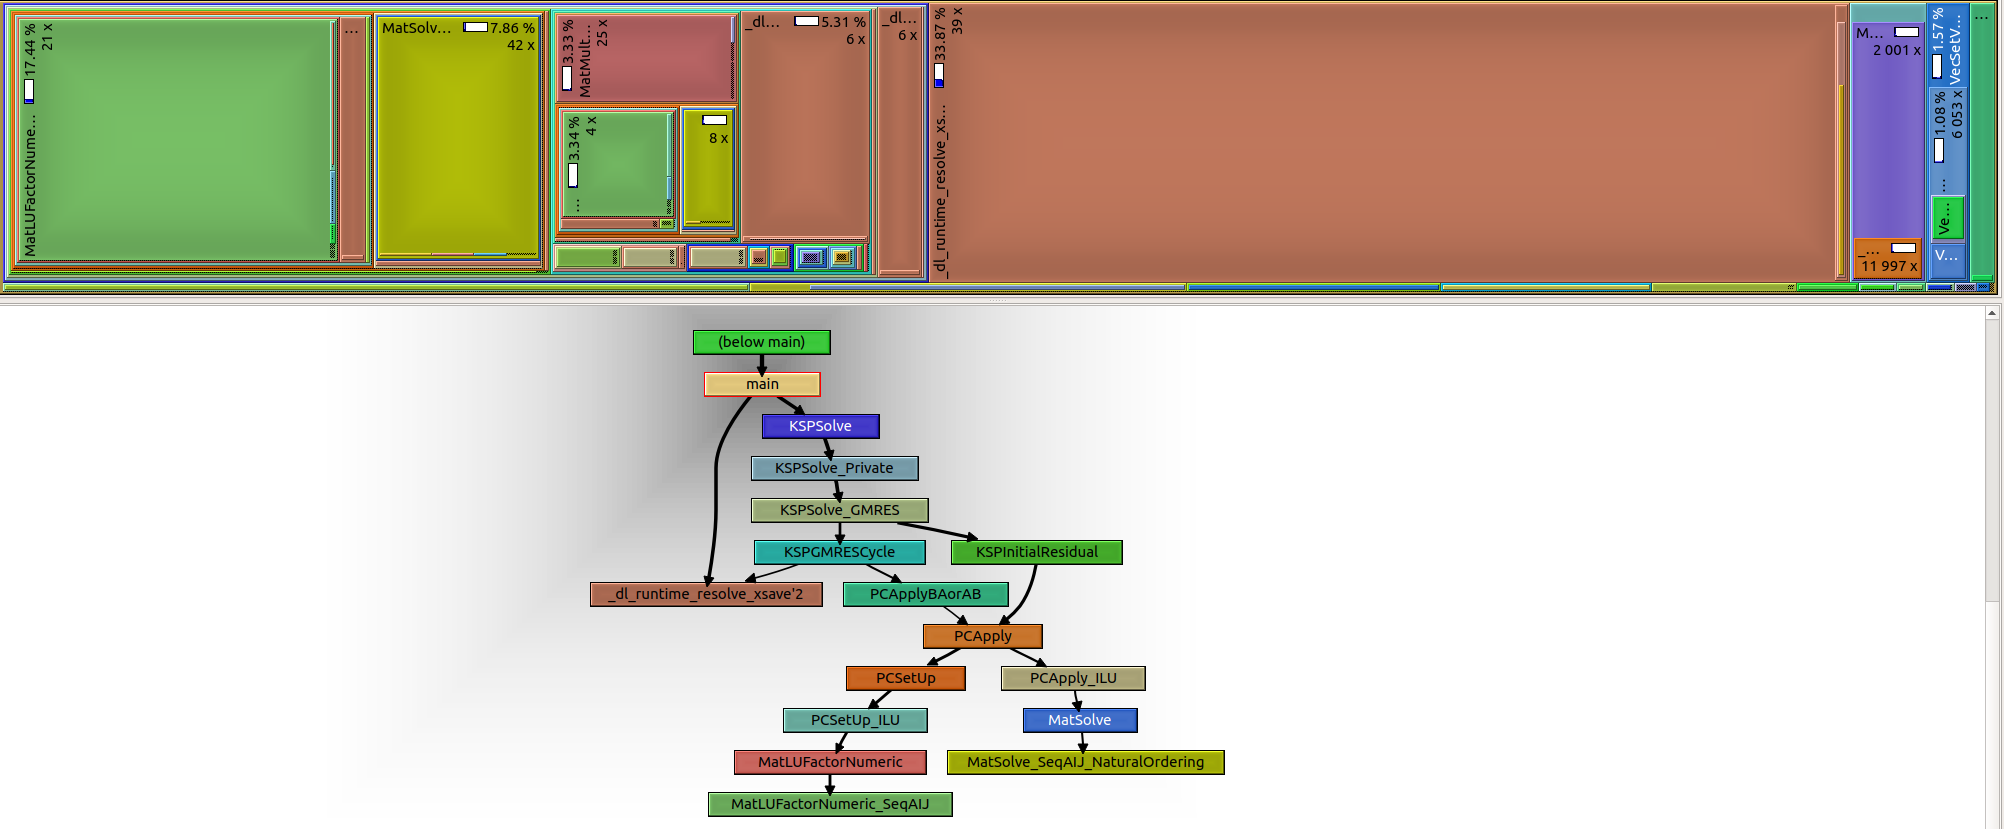
\includegraphics[angle=0, scale=0.35]{./figures/callgrind.png}
    		\end{tabular}
    	\end{center}
    	\caption{使用kcachegrind画出分析可视图:隐式}
    	\label{fig:illustration-callgrind}
    \end{figure} 

    \begin{figure}[h]
    	\begin{center}
    		\begin{tabular}{c}    			
    			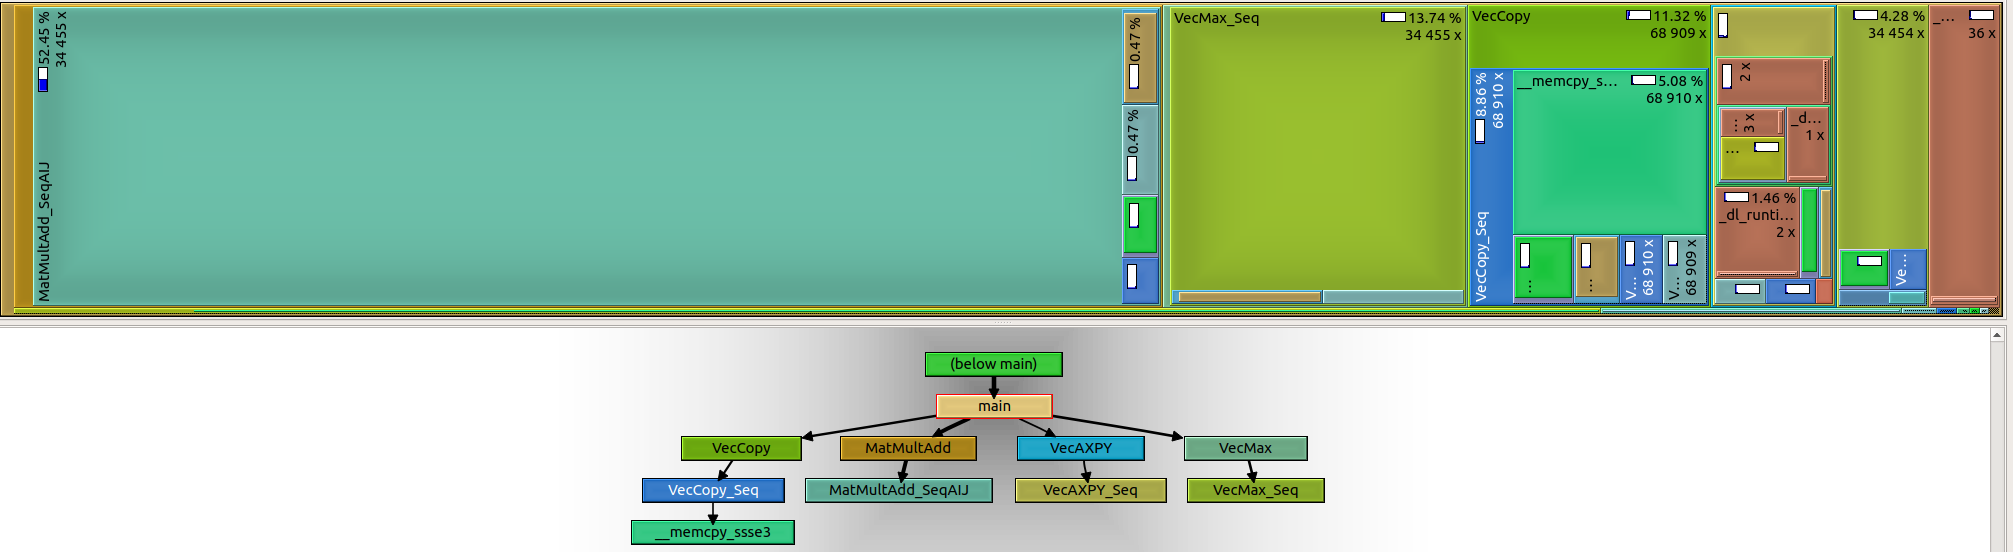
\includegraphics[angle=0, scale=0.35]{./figures/callgrind1.png}
    		\end{tabular}
    	\end{center}
    	\caption{使用kcachegrind画出分析可视图:显式}
    	\label{fig:illustration-callgrind1}
    \end{figure} 
	
	\clearpage
	
	\subsection{Visualization utility}
	
	
	\begin{figure}[h]
		\begin{center}
			\begin{tabular}{c}
				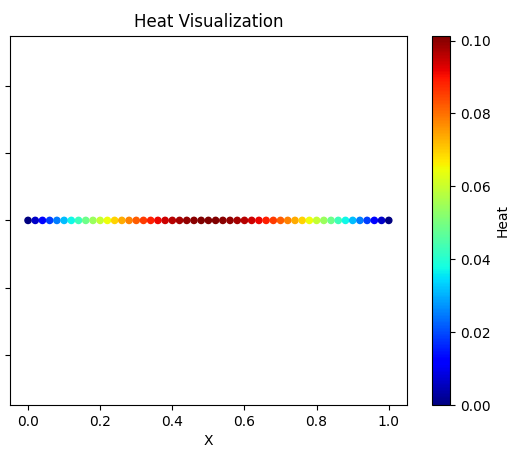
\includegraphics[angle=0, scale=0.6]{./figures/visualization.png}
			\end{tabular}
		\end{center}
		\caption{使用包含vtk库的vedo工具包,可视化热量分布}
		\label{fig:illustration-visualization}
	\end{figure}

    如上图所示,选取 50 个点,时间步取 0.0001 ,用显式欧拉迭代出温度值,并用 vedo 包含的 vtk\_python 画出可视化温度分布。
	
	\clearpage
	\section{Code testing}

	\subsection{Manufactured solution method}
	\begin{figure}[h]
		\begin{center}
			\begin{tabular}{c}
				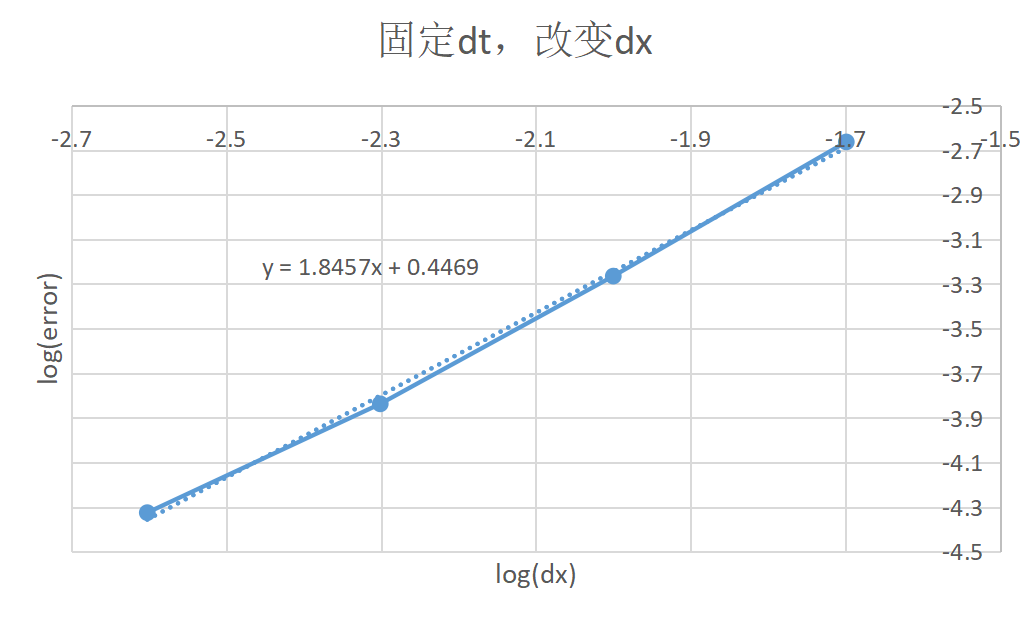
\includegraphics[angle=0, scale=0.3]{./figures/dx_coff.png}
			\end{tabular}
		\end{center}
		\caption{确定dx的幂次,这里取1.8457}
		\label{fig:illustration-dx_coff}
	\end{figure}
	\begin{figure}[h]
		\begin{center}
			\begin{tabular}{c}
				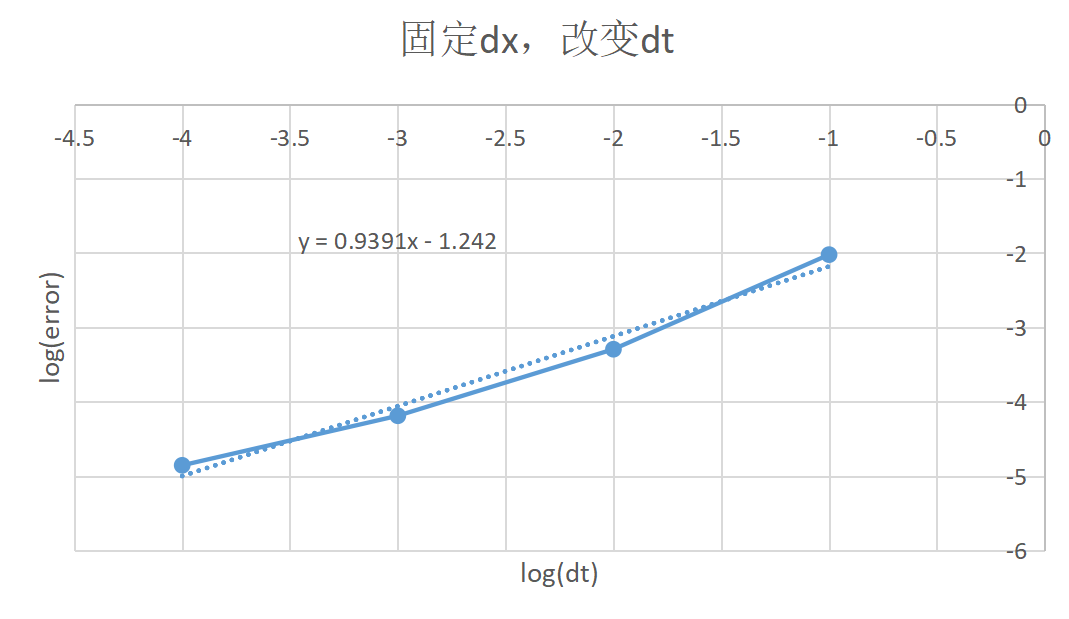
\includegraphics[angle=0, scale=0.3]{./figures/dt_coff.png}
			\end{tabular}
		\end{center}
		\caption{确定dt的幂次,这里取0.9391}
		\label{fig:illustration-dt_coff}
	\end{figure}

    

    根据精确解和隐式迭代算法所得解之间的误差,计算获得了如上的两个曲线图,
    
    拟合后取 $ \alpha = 1.8457 , \beta = 0.9391 $ ,用来估计误差 $ e \approx C_{1} \Delta x^{\alpha}+C_{2} \Delta t^{\beta} $。
    
    \clearpage
    

	\subsection{Parallelism}
	\subsubsection{Strong scaling analysis}
	对于强可扩展,设置节点数量50,时间步长0.00001,从下图可以看出,问题规模较小的时候,单核效率最高,因为这时候增加核数,运行时间反而随着CPU之间通信消耗显著增加。
	\begin{figure}[h]
		\begin{center}
			\begin{tabular}{c}
				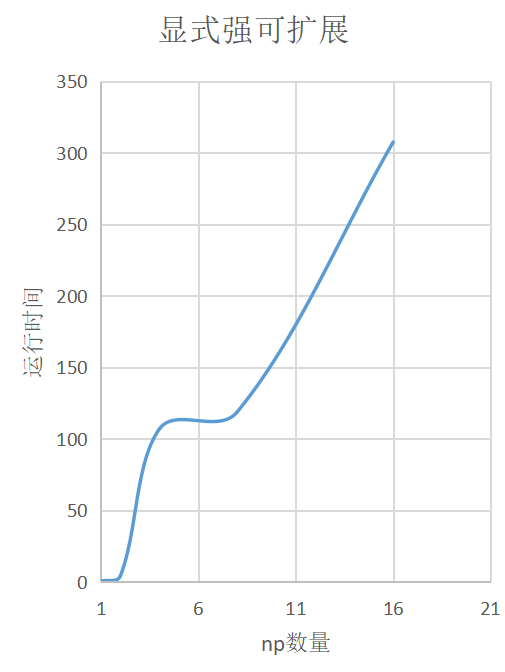
\includegraphics[angle=0, scale=0.25]{./figures/strong_ex.png}
				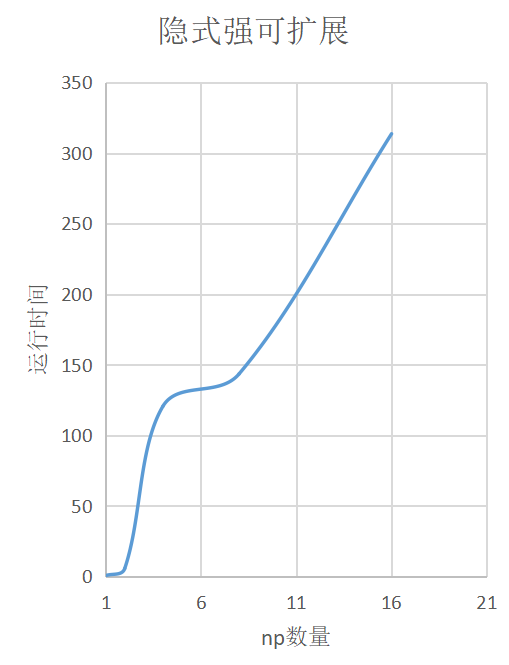
\includegraphics[angle=0, scale=0.25]{./figures/strong_im.png}
			\end{tabular}
		\end{center}
		\caption{强可扩展运行时间不减反增}
		\label{fig:illustration-strong}
	\end{figure}

    \subsubsection{Weak scaling analysis}
    对于弱可扩展,设置节点数量随着核数一同增加,如下图所示,时间步长仍然设为0.00001。和强可扩展结论一样,问题规模较小的时候,单核效率最高,多核的运行时间因为CPU之间通信耗散显著增加。
    \begin{figure}[h]
    	\begin{center}
    		\begin{tabular}{c}
    			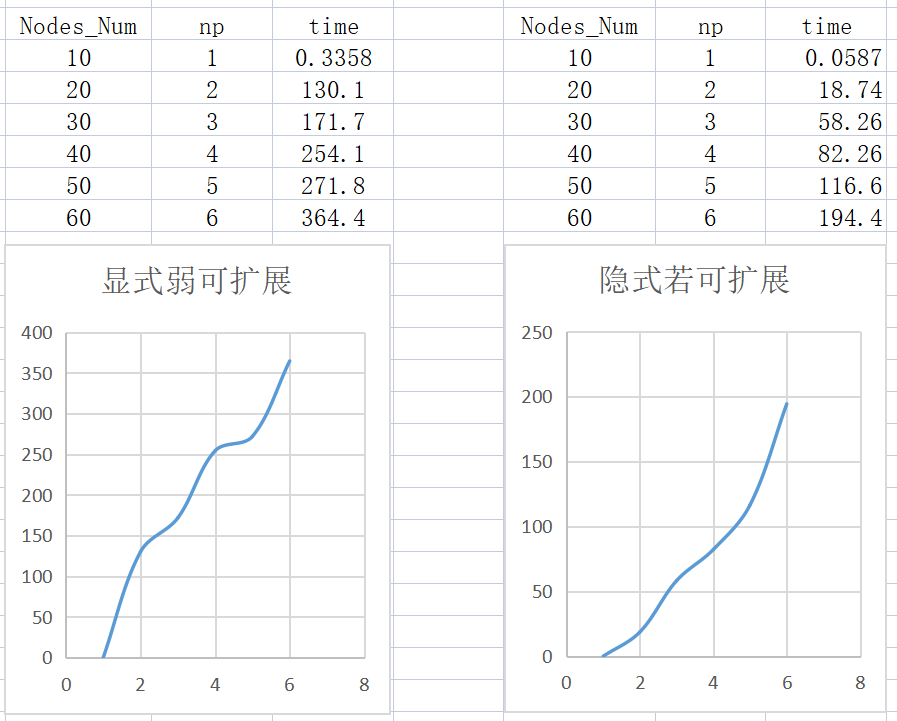
\includegraphics[angle=0, scale=0.27]{./figures/week.png}
    		\end{tabular}
    	\end{center}
    	\caption{弱可扩展运行时间不减反增,而且由于问题规模比较小,$ Nodes\_Num $节点数的增多并未对时间有显著影响}
    	\label{fig:illustration-week}
    \end{figure}

    \subsubsection{PC options}
    对于预条件子等,如下表所示,可以看出在隐式差分下,都能正确求解到要求精度前提下,lu 分解最快,ksp\_type = cg  pc\_type = jacobi 次之,它们迭代速度快,求解效率高,适合并行加速运算。
    \begin{figure}[h]
    	\begin{center}
    		\begin{tabular}{c}
    			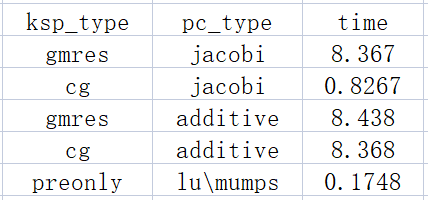
\includegraphics[angle=0, scale=0.4]{./figures/pc.png}
    		\end{tabular}
    	\end{center}
    	\caption{达到同样误差精度,lu分解速度最快}
    	\label{fig:illustration-pc}
    \end{figure}
		
	\begin{thebibliography}{99}  
		\bibitem{ref1}Recktenwald, Gerald. “Finite-Difference Approximations to the Heat Equation.” (2004).  
		\bibitem{ref2}微分方程数值解法/戴嘉尊,邱建贤编著.-南京:东南大学出版社,2002.02.-233页
	\end{thebibliography}


\end{document}

